\documentclass{article}

\usepackage{graphicx}
\usepackage{tikz}
\usepackage{tikzsymbols}
\usetikzlibrary{calc,patterns,shapes.geometric}
\pagestyle{empty}
\usepackage[margin=0pt]{geometry}
\geometry{papersize={14in,12in}}

\def\centerarc[#1](#2)(#3:#4:#5){\draw[#1] ($(#2)+({#5*cos(#3)},{#5*sin(#3)})$) arc (#3:#4:#5);}

\begin{document}
	\begin{figure}
		\centering
		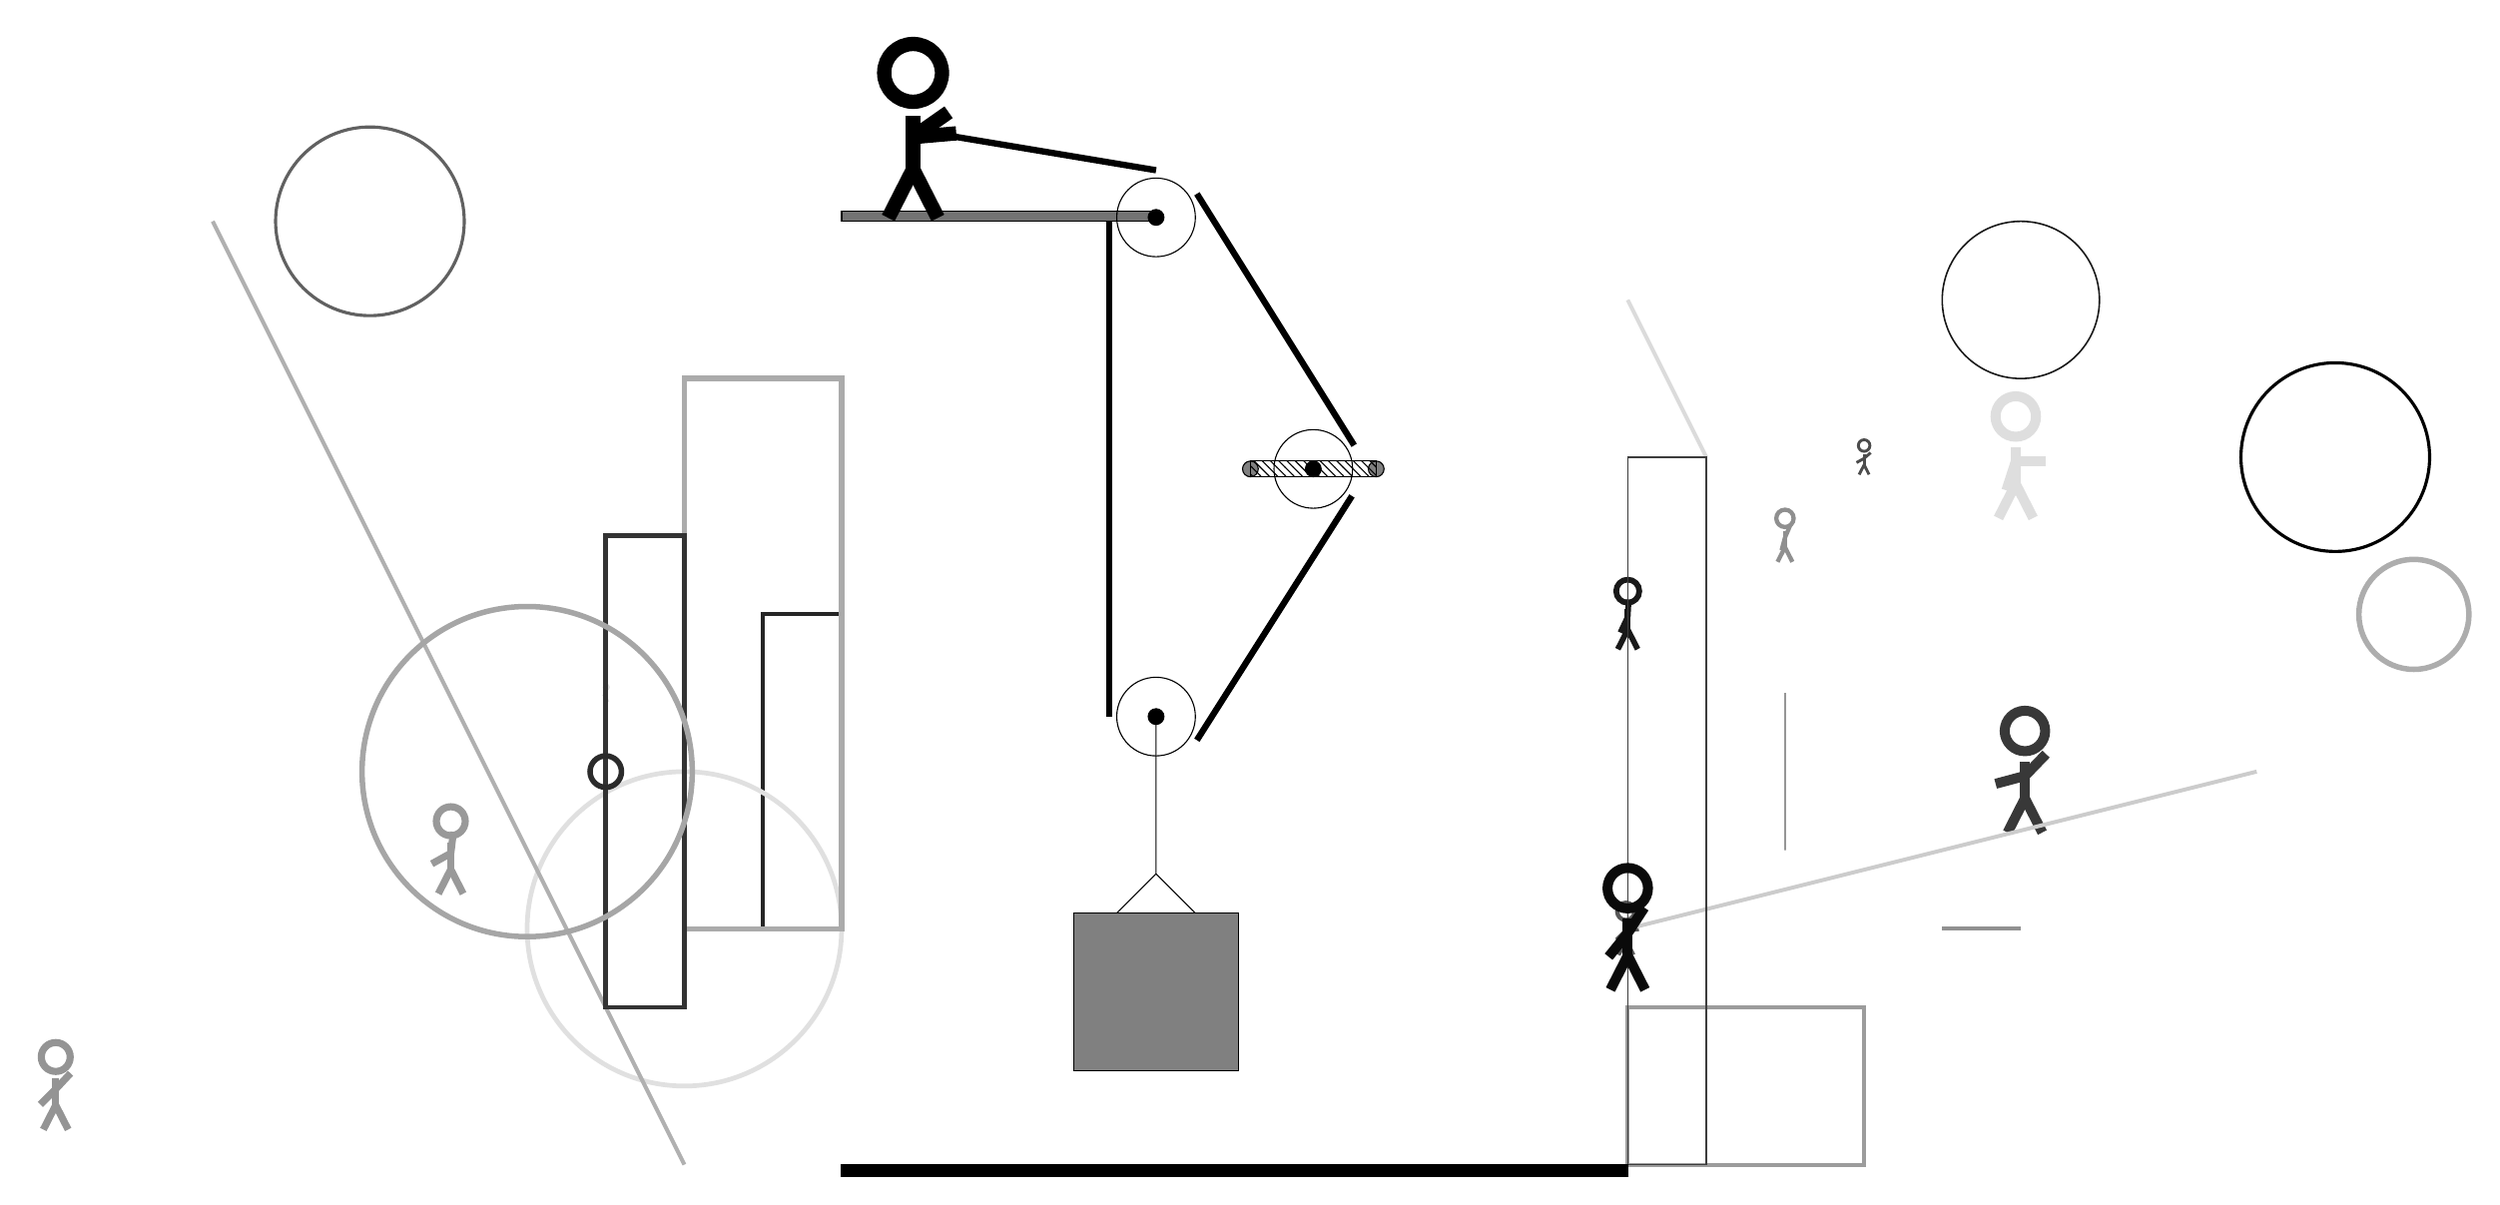
\begin{tikzpicture}
			%%%%% START %%%%%
			
			\draw[fill=black!55] (-2, 9) rectangle (2, 9.125);
			
			\draw (2, 2.7) circle (0.5);
			\draw[fill=black] (2, 2.7) circle (0.1);
			
			\draw (2, 9.05) circle (0.5);
			\draw[fill=black] (2, 9.05) circle (0.1);
			
			\node[line width=0.5mm, color=black!78] at (13, 2) {\Strichmaxerl[7][15][46]};
			
			\node[line width=0.3mm, color=black!42] at (-12, -2) {\Strichmaxerl[5][45][47]};
			\draw[line width=0.5mm, color=black!85] (-3, 4) rectangle (-2, 0);
			\draw [line width=0.6mm, color=black!12](-4, 0) circle (2.0);
			\draw[line width=0.5mm, color=black!43](13, 0) -- (12, 0);
			
			\node[line width=0.4mm, color=black!65] at (8, 0) {\Strichmaxerl[3][45][7]};
			\draw[line width=0.5mm, color=black!39] (8, -1) rectangle (11, -3);
			\draw [line width=0.4mm, color=black!100](17, 6) circle (1.2);
			\node[line width=0.4mm, color=black!13] at (13, 6) {\Strichmaxerl[7][72][0]};
			
			\node[line width=0.6mm, color=black!90] at (8, 4) {\Strichmaxerl[4][65][87]};
			\draw[line width=0.7mm, color=black!33] (-2, 0) rectangle (-4, 7);
			
			\draw [line width=0.4mm, color=black!62](-8, 9) circle (1.2);
			\node[line width=0.2mm, color=black!70] at (11, 6) {\Strichmaxerl[2][29][41]};
			
			\draw[line width=0.5mm, color=black!14](8, 8) -- (9, 6);
			\draw[line width=0.5mm, color=black!31](-4, -3) -- (-10, 9);
			\node[line width=0.6mm, color=black!44] at (10, 5) {\Strichmaxerl[3][75][67]};
			
			\node[line width=0.4mm, color=black!11] at (-5, 3) {\Strichmaxerl[1][26][80]};
			
			\draw[line width=0.5mm, color=black!20](8, 0) -- (16, 2);
			\draw[line width=0.3mm, color=black!41] (10, 3) rectangle (10, 1);
			\draw[line width=0.2mm, color=black!81] (8, -2) rectangle (8, 3);
			\draw[line width=0.6mm, color=black!80] (-4, 5) rectangle (-5, -1);
			\draw [line width=0.7mm, color=black!35](-6, 2) circle (2.1);
			\draw [line width=0.7mm, color=black!32](18, 4) circle (0.7);
			\draw[line width=0.2mm, color=black!76] (9, -3) rectangle (8, 6);
			\draw [line width=0.7mm, color=black!83](-5, 2) circle (0.2);
			\draw [line width=0.2mm, color=black!91](13, 8) circle (1.0);
			\node[line width=0.3mm, color=black!96] at (8, 0) {\Strichmaxerl[7][51][57]};
			\node[line width=0.6mm, color=black!40] at (-7, 1) {\Strichmaxerl[5][29][83]};
			
			\draw[fill=white](4, 5.85) circle (0.5);
			\draw[fill=black] (4, 5.85) circle (0.1);
			\draw[fill=black!50] (3.2, 5.85) circle (0.1);
			\draw[fill=black!50] (4.8, 5.85) circle (0.1);
			\draw[pattern=north west lines, pattern color=black] (3.2, 5.95) rectangle (4.8, 5.75);
			
			\draw (2, 2.7) -- (2, 0.7) -- (1.5, 0.2) -- (2.5, 0.2) -- (2, 0.7);
			\draw[fill=black!50] (0.95, 0.2) rectangle (3.05, -1.8);
			
			\draw[line width=0.8mm] (1.4, 9) -- (1.4, 2.7);
			\centerarc[line width=0.8mm](2, 2.7)(180:330:0.6);
			\draw[line width=0.8mm](2.5196, 2.4) -- (4.4915, 5.5058);
			\centerarc[line width=0.8mm](4, 5.85)(390:325:0.6);
			\draw[line width=0.8mm](4.5196, 6.15) -- (2.5196, 9.35);
			\centerarc[line width=0.8mm](2, 9.05)(30:90:0.6);
			\draw[line width=0.8mm](2, 9.65) -- (-1, 10.15);
			
			\node at (-1, 10.15) {\Strichmaxerl[10][-175][35]};
			
			\draw[fill=black] (-2, -3) rectangle (8, -3.15);
			
			%%%%% END %%%%%
		\end{tikzpicture}
	\end{figure}	
\end{document}